%%%%%%%%%%%%%%%%%%%%%%%%%%%%%%%%%%%%%%%%%
% Beamer Presentation
% LaTeX Template
% Version 1.0 (10/11/12)
%
% This template has been downloaded from:
% http://www.LaTeXTemplates.com
%
% License:
% CC BY-NC-SA 3.0 (http://creativecommons.org/licenses/by-nc-sa/3.0/)
%
%%%%%%%%%%%%%%%%%%%%%%%%%%%%%%%%%%%%%%%%%

%----------------------------------------------------------------------------------------
%	PACKAGES AND THEMES
%----------------------------------------------------------------------------------------

\documentclass{beamer}
\mode<presentation> {

% The Beamer class comes with a number of default slide themes
% which change the colors and layouts of slides. Below this is a list
% of all the themes, uncomment each in turn to see what they look like.

%\usetheme{default}
%\usetheme{AnnArbor}
% %\usetheme{Antibes}
%\usetheme{Bergen}
%\usetheme{Berkeley}
%\usetheme{Berlin}
%\usetheme{Boadilla}
%\usetheme{CambridgeUS}
%\usetheme{Copenhagen}
%\usetheme{Darmstadt}
%\usetheme{Dresden}
%\usetheme{Frankfurt}
%\usetheme{Goettingen}
%\usetheme{Hannover}
%\usetheme{Ilmenau}
%\usetheme{JuanLesPins}
%\usetheme{Luebeck}
\usetheme{Madrid} %%%%
%\usetheme{Malmoe}
%\usetheme{Marburg}
%\usetheme{Montpellier}
%\usetheme{PaloAlto}
%\usetheme{Pittsburgh}
%\usetheme{Rochester}
%\usetheme{Singapore}
%\usetheme{Szeged}
%\usetheme{Warsaw}

% As well as themes, the Beamer class has a number of color themes
% for any slide theme. Uncomment each of these in turn to see how it
% changes the colors of your current slide theme.

%\usecolortheme{albatross}
%\usecolortheme{beaver}
%\usecolortheme{beetle}
%\usecolortheme{crane}
%\usecolortheme{dolphin}
%\usecolortheme{dove}
%\usecolortheme{fly}
%\usecolortheme{lily}
%\usecolortheme{orchid}
%\usecolortheme{rose}
%\usecolortheme{seagull}
%\usecolortheme{seahorse}
%\usecolortheme{whale}
%\usecolortheme{wolverine}

%\setbeamertemplate{footline} % To remove the footer line in all slides uncomment this line
%\setbeamertemplate{footline}[page number] % To replace the footer line in all slides with a simple slide count uncomment this line

%\setbeamertemplate{navigation symbols}{} % To remove the navigation symbols from the bottom of all slides uncomment this line
}

\usepackage{graphicx} % Allows including images
\usepackage{graphics}
\usepackage{booktabs} % Allows the use of \toprule, \midrule and \bottomrule in tables
\usepackage[english, french]{babel}  %support francais et anglais
\usepackage[utf8]{inputenc}
%\bibliographystyle{plainnat}
%\bibliography{cdansereau}


%----------------------------------------------------------------------------------------
%	TITLE PAGE
%----------------------------------------------------------------------------------------

\title[Schizophrenia classification]{Schizophrenia classification using \\multi-scale functional connectivity } % The short title appears at the bottom of every slide, the full title is only on the title page

\author{Christian Dansereau} % Your name
\institute[DIRO] % Your institution as it will appear on the bottom of every slide, may be shorthand to save space
{
Université de Montréal \\ % Your institution for the title page
\medskip
%\textit{john@smith.com} % Your email address
}
\date{28 Avril 2015} % Date, can be changed to a custom date

\begin{document}

\begin{frame}
\titlepage % Print the title page as the first slide
\end{frame}

%\begin{frame}
%\frametitle{Overview} % Table of contents slide, comment this block out to remove it
%\tableofcontents % Throughout your presentation, if you choose to use \section{} and \subsection{} commands, these will automatically be printed on this slide as an overview of your presentation
%\end{frame}

%----------------------------------------------------------------------------------------
%	PRESENTATION SLIDES
%----------------------------------------------------------------------------------------

%------------------------------------------------
\section{Contexte général} 
%------------------------------------------------
\frame{\sectionpage}
%------------------------------------------------
%\subsection{Imagerie par résonance magnétique fonctionnelle} 
%------------------------------------------------

\begin{frame}
\frametitle{Imagerie par résonance magnétique (IRM)}
\begin{figure}
\begin{center}
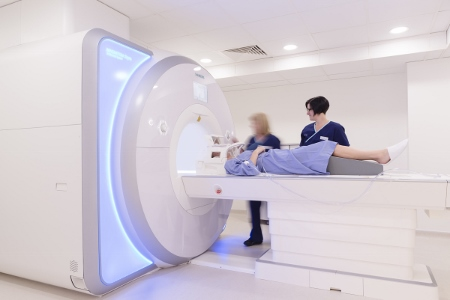
\includegraphics[width=0.7\linewidth]{../figures/scanner.jpg}
\end{center}
\end{figure}
\end{frame}


\begin{frame}
\frametitle{IRM fonctionnelle (IRMf)}
\begin{figure}[H]
\begin{center}
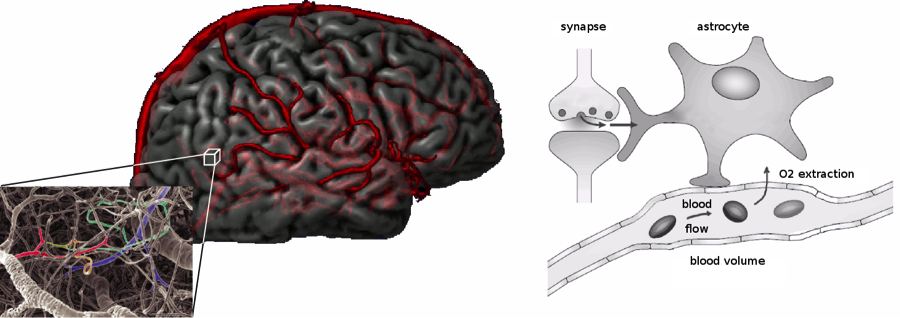
\includegraphics[width=\linewidth]{../figures/bold.png}
\end{center}
\tiny{Adapté de Heeger 2002.}
\end{figure}
\end{frame}

%------------------------------------------------
%\subsection{Prétraitement} 
%------------------------------------------------
\begin{frame}
\frametitle{Preprocessing de l'IRMf}
\begin{figure}[H]
\begin{center}
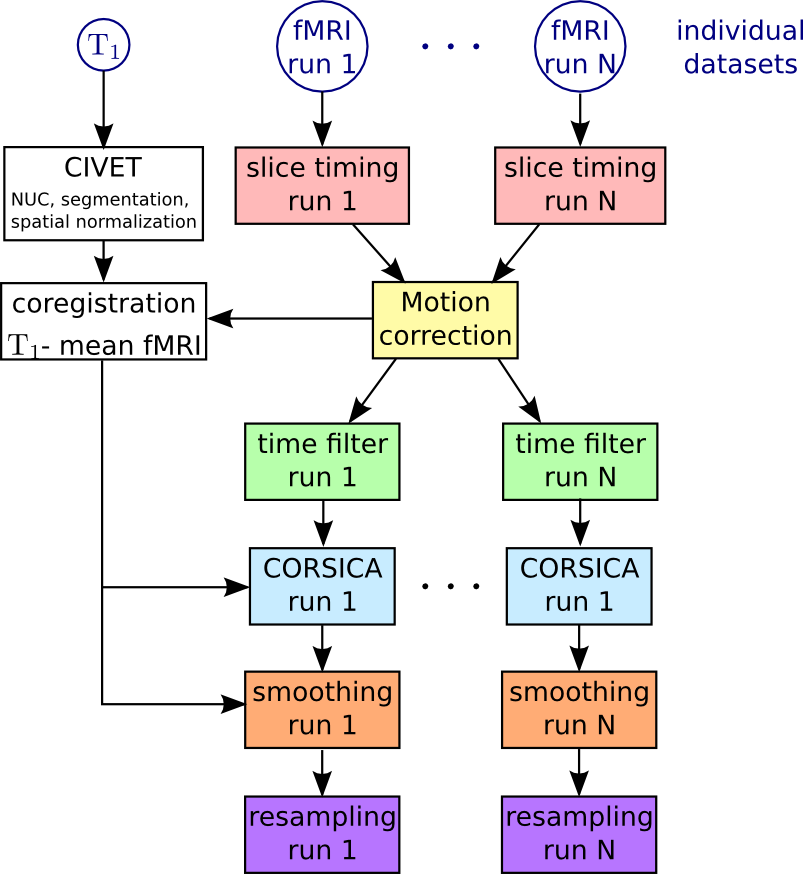
\includegraphics[scale=0.6]{../figures/fig_flowchart_fmri_preprocess.png}
\end{center}
\end{figure}
\tiny{\url{http://www.nitrc.org/projects/niak/}}
\end{frame}



\begin{frame}
\frametitle{Connectome}
\begin{figure}
\begin{center}
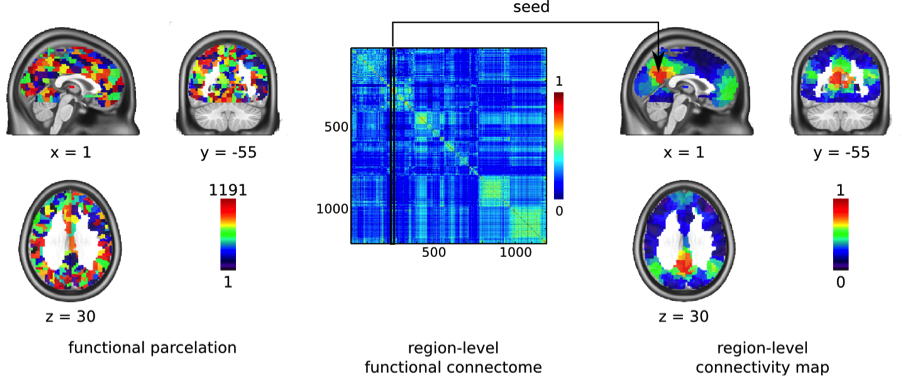
\includegraphics[scale=0.8]{../figures/connectome.png}
\end{center}
\tiny{(``Neuroimaging Analysis Kit'' (NIAK) \footnote{\url{http://www.nitrc.org/projects/niak/}}).}
\label{fig_motion_estimation}
\end{figure}
\end{frame}


\begin{frame}
\frametitle{Multiscale connectomes}
\begin{figure}
\begin{center}
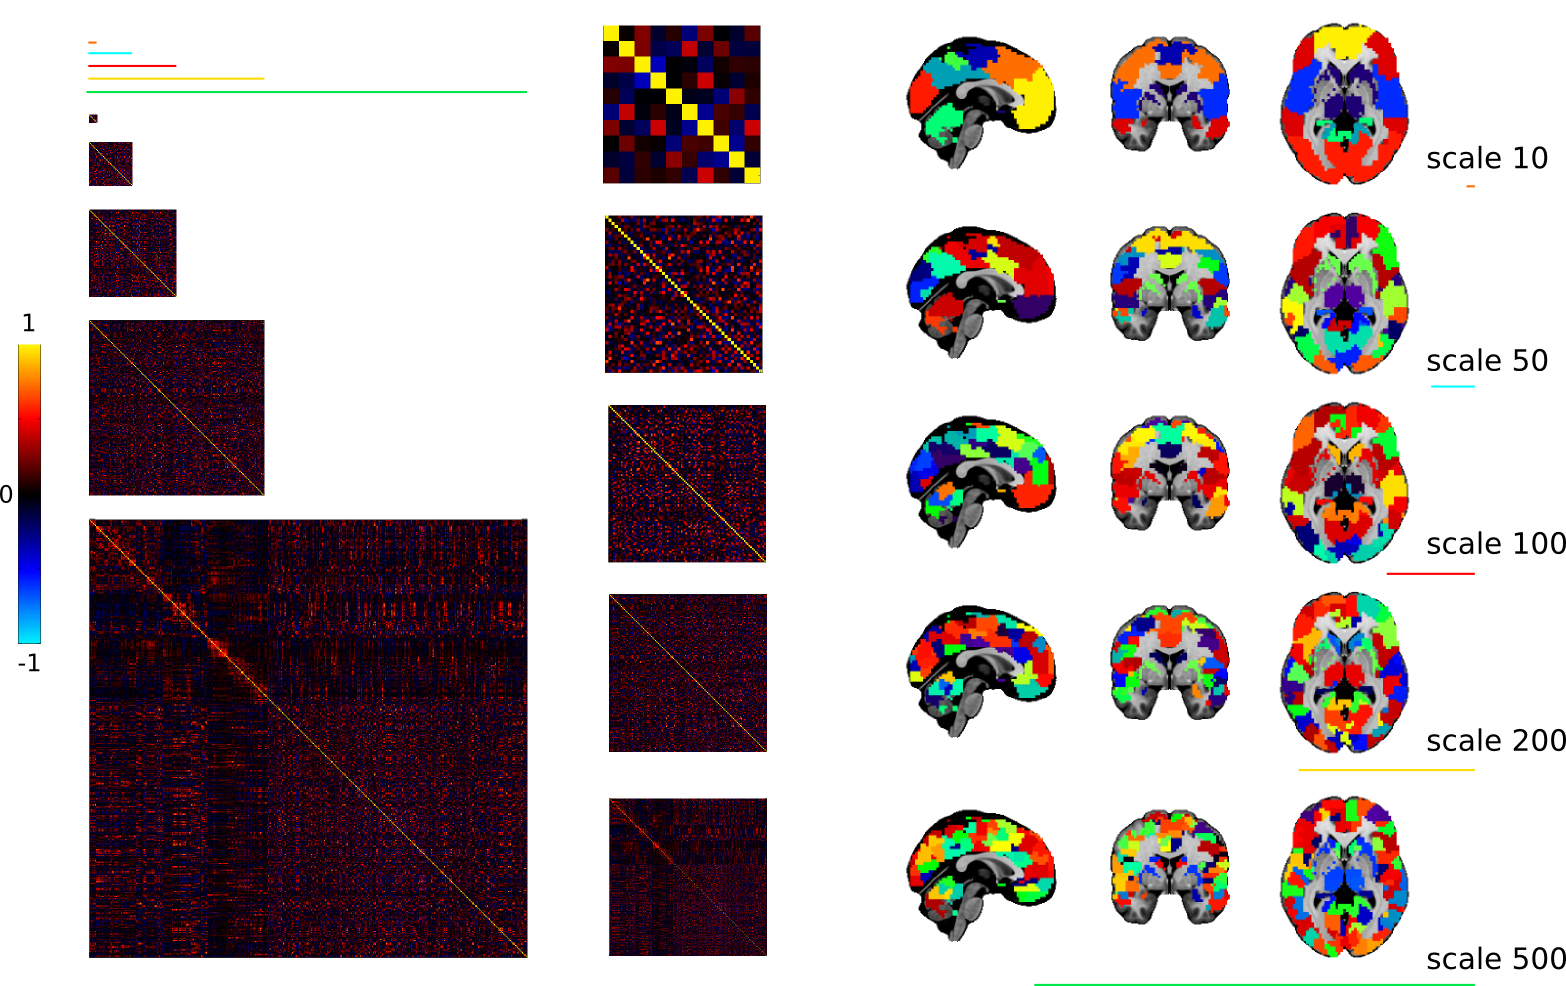
\includegraphics[scale=0.5]{../figures/fig_connectome_multiscale.png}
\end{center}
\tiny{Multiscale connectomes.}
\label{fig_multiscale}
\end{figure}
\end{frame}




\frame{
\frametitle{Jeux de donnée}
COBRE\footnote{\url{http://fcon_1000.projects.nitrc.org/indi/retro/cobre.html}} (The Center for Biomedical Research Excellence)
\hfill\break
Total: 147 sujets
\begin{itemize}
\item 72 patients atteints de schizophrénie 
\item 75 contôles
\item Donnée phenotypic (age, genre, diagnostique)
\item âge = 18-65
\end{itemize}
\hfill\break
}

\begin{frame}
\frametitle{Multiscale connectomes COBRE}
\begin{figure}
\begin{center}
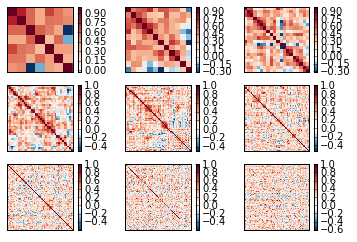
\includegraphics[scale=0.9]{../figures/connectome3x3.png}
\end{center}
\tiny{Multiscale connectomes COBRE (7, 12, 20, 36, 64, 122, 197, 325 and 444).}
\label{fig_multiscale_cobre}
\end{figure}
\end{frame}

%------------------------------------------------
\section{Méthod}
%------------------------------------------------
\frame{\sectionpage}

\begin{frame}
\frametitle{1) Structure du pipeline d'analyse}
\hfill\break
\begin{itemize}
\item 10-fold Crossvalidation
\item Normalisation
\item Régression des composantes de non-intérêt
\item Optimisation des parametres du SVM (C et Gamma)
\end{itemize}
\end{frame}

\begin{frame}
\frametitle{2) Bagging multiéchelle}
\begin{figure}
\begin{center}
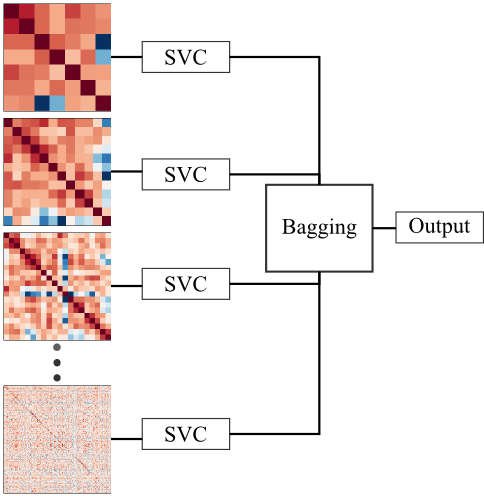
\includegraphics[scale=1.]{../figures/bagging_multiscale.png}
\end{center}
\end{figure}
\end{frame}

\begin{frame}
\frametitle{3) Sélection d'attribut par maximisation de la marge}
\begin{figure}
\begin{center}
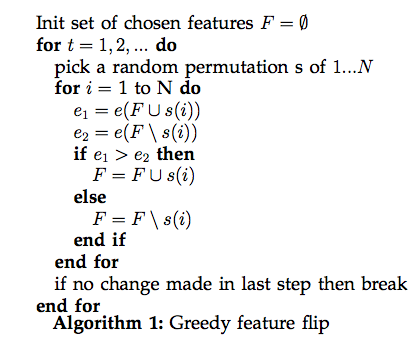
\includegraphics[scale=.5]{../figures/gflip.png}
\end{center}
\end{figure}
\tiny{Gilad-bachrach et al. 2004}
\end{frame}

%------------------------------------------------
\section{Résultats}
%------------------------------------------------
\frame{\sectionpage}

\begin{frame}
\frametitle{Calibration}
\begin{figure}
\begin{center}
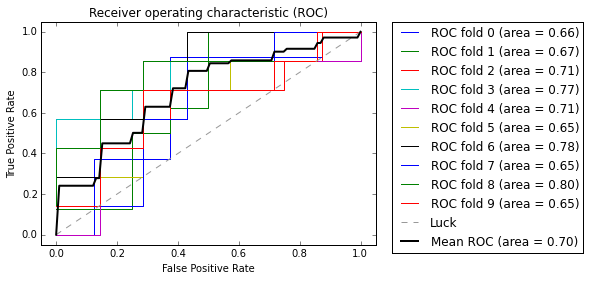
\includegraphics[scale=.5]{../figures/svc_linear_calibration_scale64x64.png}
\end{center}
\end{figure}
\tiny{SVC linear, C=1 , 64x64 scale}
\end{frame}



\begin{frame}
\frametitle{Optimisation de l'échelle}
\begin{figure}
\begin{center}
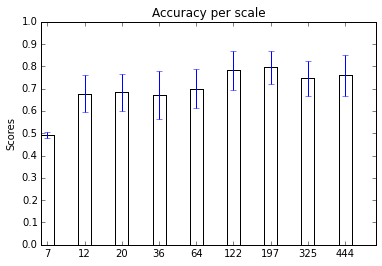
\includegraphics[scale=0.7]{../figures/acc_scale.png}
\end{center}
\tiny{Précision de chaque échelle}
\label{fig_multiscale_cobre}
\end{figure}
\end{frame}


\begin{frame}
\frametitle{Sommaire des résultats}
\begin{table}[h]
\begin{tabular}{llll}
\hline
                                   & Accuracy (\%)  & Std (\%)      & AUC           \\ \hline
SVC linear calib 64x64             & 64.53          & 6.86          & 0.70          \\
NC SVC linear 64x64                & 67.07          & 11.08         & 0.75          \\
Opt NC SVC linear 64x64            & 69.89          & 8.69          & 0.80          \\
\textbf{Opt NC SVC linear 197x197} & \textbf{79.48} & \textbf{7.50} & \textbf{0.82} \\
Opt NC SVC rbf 197x197             & 74.61          & 8.75          & 0.80          \\
\textbf{Opt NC multiscale bagging} & \textbf{80.14} & \textbf{8.36} & \textbf{0.82} \\
Opt NC I-Relief 197x197            & 73.94          & 7.41          & 0.82          \\ \hline
\end{tabular}
\label{tab_results}
\tiny{Acronyms: calib: calibration, NC: normalized and regression of confounds (age and gender), Opt: optimisation of the classification parameter using nested 10-fold cross-validation. The multiscale bagging was performed on 3 scales (122, 197 and 444) and I-Relief was perform on the scale 197. }
\end{table}
\end{frame}

%------------------------------------------------
\section{Conclusion}
%------------------------------------------------
\frame{\sectionpage}

\begin{frame}
\frametitle{Conclusion}

\hfill\break
\begin{itemize}
\item Autre model exploré: SVM with Gaussian kernel, LDA, Adaboost, Bagging, trees et random forest
\item Bonne performance pour un problème assez difficile (80\%).
\item Bagging multiéchelle est probablement une meilleure idée.
\item Généralisation à d'autres jeux de donnée et pathologie.
\end{itemize}
\end{frame}

%----------------------------------------------------------------------------------------

\begin{frame}
\Huge{\centerline{Merci}}
\end{frame}

%----------------------------------------------------------------------------------------


\end{document} 